\documentclass[11pt]{article}
\title{Symmetry 9}
\author{https://github.com/heptagons/lenses}
\date{2024/1/25}

\usepackage{graphicx}
\usepackage{amsfonts,amsmath,amssymb,amsthm}

\usepackage[margin=0.75in]{geometry}
\usepackage{float} % {figure}{H}
\usepackage{amsmath} % \dfrac

\def\mathbi#1{\textbf{\em #1}}

\begin{document}

\maketitle
\begin{abstract}
The define odd symmetry $s=\{ 3,5,7,9,... \}$ as the set of pairs of lines of length $1$ connected at their vertices and forming angles equal to $2\pi u/s, u = 1,2,...,s-1$. We study here symmetry $s=9$ and found the lines can form hexagons, octagons and grater equilateral polygons.
\end{abstract}

\section{Symmetries}

We are interested in odd symmetries starting with $s=3$. Table \ref{tbl:symm} show the symmetries up to $s=9$. The minimum possible angle of the symmetry $s$ is $\theta = \dfrac{2\pi}s$. 

\begin{table}[H]
\begin{center}
\begin{tabular}{|c|c c|}
\hline
$s$ & Angle $\theta$ & Minimal value \\ \hline\
$3$ & $\alpha$ & $2\pi/3$ \\ \hline
$5$ & $\beta$  & $2\pi/5$ \\ \hline
$7$ & $\gamma$ & $2\pi/7$ \\ \hline
$9$ & $\delta$ & $2\pi/9$ \\ \hline
\end{tabular}
\caption{Angles of symmetries $s=\{3,5,7,9\}$.} 
\label{tbl:symm}
\end{center}
\end{table}

Let $t = \dfrac{s+1}2$. We define $t$ independent abscissas and ordinates $x_i, y_i$ as follows:
\begin{align}
\left[ \begin{array}{c} x_i \\ y_i \end{array} \right] &= 
\left[ \begin{array}{c} \cos((i-1)\theta) \\ \sin((i-1)\theta) \end{array} \right]
 \quad i = 1,2,...,t \label{eq:pairs}
\end{align}

Let define a point $p_0$ located at coordinates $(0,0)$. Then there are exactly $s$ different points $p_1, p_2, ... p_s$  equidistant to point $p_0$ located at coordinates $\langle x_i,y_i \rangle$ as follows:
\begin{align}
p_i &\equiv \left\{ \begin{array}{ccl}
 \langle x_j,y_j\rangle & \mbox{for} & i \leq t  \quad j = i\\
 \langle x_j, -y_j\rangle & \mbox{for} & i > t \quad j = s+2-i
 \end{array}\right. \label{eq:coords}
\end{align}

We transform each point $p_i$ into a vector $v_i$ which holds only the $(x,y)$ pair of indices and the signs:
\begin{align}
v_i &\equiv \left\{ \begin{array}{ccl}
 ( j, j ) & \mbox{for} & i \leq t \quad j = i\\
 ( j, -j ) & \mbox{for} & i > t \quad j = s+2-i
 \end{array}\right. \label{eq:vectors}
\end{align}

Any vector $v_i \equiv (k_1,k_2)$ can be rotated by $180^\circ$ around $p_0$. The vector after the rotation is denoted as $\overline{v_i}$ and the original indices $k_1,k_2$ signs are changed:
\begin{align}
\overline{v_i} &\equiv (-k_1, -k_2) \label{eq:vector180}
\end{align}

Lets build lines and connect them to form a \textbf{polyline}. First we start at the vertice $o$ located at coordinates $(0,0)$ and add vectors alternating the type $v_i$ and the type $\overline{v_i}$ in order the angles at the vertices are multiples of $\theta$. For example, the polyline with vectors $\overrightarrow{P_1P_2}=v_a$, $\overrightarrow{P_2P_3}=\overline{v_b}$, $\overrightarrow{P_3P_4}=v_c$, ... is denoted as:
\begin{align}
\overline{P_1P_2P_3P_4...} &= \{ [], [v_a], [v_a,\overline{v_b}],[v_a,\overline{v_b},v_c],... \} 
 & 1 \leq a,b,c \leq t \\
 &= P_s(0,a,b,c,...) & \mbox{simplifyed form}
\end{align}

For two consecutive points $P_k = [...,v_m]$ and $P_{k+1} = [...,v_m,\overline{v_n}]$ for $k>0$ we have that the angle at point $P_k$ is $u\theta$, where $u$ is:
\begin{align}
u &\equiv s + m - n \pmod{s} \quad  \quad 1 \leq m,n \leq t \label{eq:angle}
\end{align}

Every point can be located independently by pre-calculating \textbf{accumulators} $\textbf{P}^S$ wich are integer matrices of size $t\times 2$:
\begin{align}
\textbf{X} &= \left[\begin{array}{ccccc}X_1&X_2&X_3&...&X_t
 \end{array}\right]  \quad X_i \in \mathbb{Z}\\
\textbf{Y} &= \left[\begin{array}{ccccc}Y_1&Y_2&Y_3&...&Y_t
 \end{array}\right]  \quad Y_i \in \mathbb{Z}\\
\textbf{P}^A &\equiv \left[\begin{array}{c}\textbf{X} \\ \textbf{Y}
 \end{array}\right]
 = \left[\begin{array}{ccccc}X_1&X_2&X_3&...&X_t
  \\ Y_1&Y_2&Y_3&...&Y_t \end{array}\right] \label{eq:accums}
\end{align}

Within the polyline accumulators are copied from previous points and incremented by $+1$ or decremented by $-1$ depending in the indices of the vector $v = (k_x,k_y)$:
\begin{align}
X_i &= \left\{ \begin{array}{ccl}
 X_i + 1 & \mbox{for} & i = k_x \\
 X_i - 1 & \mbox{for} & i = -k_x
 \end{array}\right. \\
Y_i &= \left\{ \begin{array}{ccl}
 Y_i + 1 & \mbox{for} & i = k_y \\
 Y_i - 1 & \mbox{for} & i = -k_y
 \end{array}\right.
\end{align}

The coordinates of point $P$ in $\mathbb{R}^2$ is calculated adding the products of the accumulators $\textbf{P}^A$ of equation \ref{eq:accums} and the coordinates of points $p_i$ of equation \ref{eq:coords}:
\begin{align}
\langle P_x,P_y\rangle &= 
 \biggl< \sum_{i=1}^{t}X_ix_i, \sum_{i=1}^{t}Y_iy_i \biggr> \label{eq:absolute}
\end{align}




\section{Symmetry $m=9$}

Figure \ref{fig:vectors-a} $(i)$ show the nine different vectors $v_1$, $v_2$, ... $v_9$ in symmetry $m=9$. Using the vectors equation \ref{eq:vectors} we get the nine vectors:
$v_1 = (1,1)$,
$v_2 = (2,2)$,
$v_3 = (3,3)$,
$v_4 = (4,4)$,
$v_5 = (5,5)$,
$v_6 = (11-6,-(11-6)) = (5,-5)$,
$v_7 = (11-7,-(11-7)) = (4,-4)$,
$v_8 = (11-8,-(11-8)) = (3,-3)$ and
$v_9 = (11-9,-(11-9)) = (2,-2)$.

\begin{figure}[H]
\centering
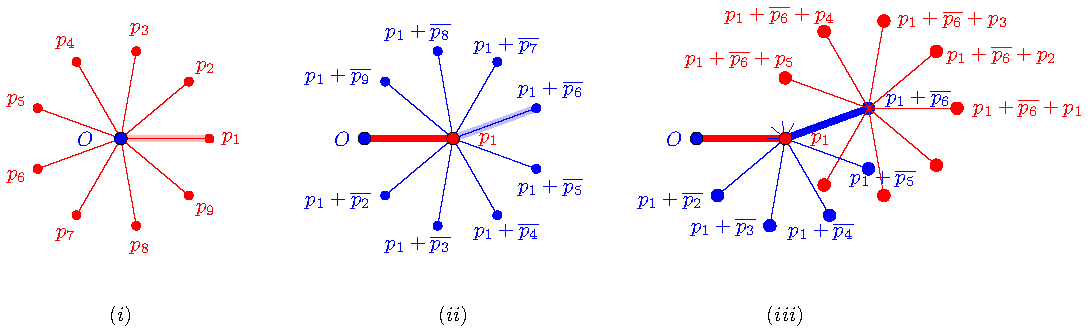
\includegraphics[scale=1]{vectors-a}
\caption{The symmetry $9$ vectors, points, angles and polylines.}
\label{fig:vectors-a}
\end{figure}

Figure \ref{fig:vectors-a} $(ii)$ show polyline $\overline{ABC}$ and $(iii)$ show polyline $\overline{ABCD}$ alternating vectors of the type $[...,v_m]$ (show in red) with vectors of the type $[...,v_m,\overline{v_n}]$ (shown in blue) to guarantee the angles between edges are always multiples of $\delta$: angle $\angle{ABC} = 4\delta$, angle $\angle{BCD} = 2\delta$. The polyline $\{A,B,C,D\}$ is denoted by $\{ [\hspace{2pt}], [v_1], [v_1, \overline{v_6}], [v_1,\overline{v_6},v_2] \}$ or in compact form $V_9(0,1,6,2)$.
\\
\\
The vertice $o$ at the origin is assigned with accumulators $\textbf{X},\textbf{Y}$ initialized to zero. For the next point the accumulators are updated at positions $1 \leq k \leq t$ according the components of the vector $v_m\equiv(k_x,k_y)$ of the new point:

\begin{align}
X[a,b,c,d,e] + v_i &= \left\{ \begin{array}{ccl}
 X[a+1,b,c,d,e] & \mbox{for} & v_1\equiv(1,1) \\
 X[a,b+1,c,d,e] & \mbox{for} & v_2\equiv(2,2), v_9\equiv(2,-2)\\
 ... & & \\
 X[a,b,c,d,e+1] & \mbox{for} & v_5\equiv(5,5), v_6\equiv(5,-5)\\
 X[a-1,b,c,d,e] & \mbox{for} & \overline{v_1}\equiv(-1,-1) \\
 ... & &
 \end{array}\right.
\end{align}

Lets get the accumulators of the polyline $\{[\hspace{2pt}], [v_1], [v_1,\overline{v_6}], [v_1,\overline{v_6},v_4]\}$ shown in figure $(iii)$. By definition the accumulators at $o \equiv (0,0)$ which is point $A=[\hspace{2pt}]$ are:
\begin{align}
[\hspace{2pt}]^A &= \left[\begin{array}{ccccc}0&0&0&0&0 \\ 0&0&0&0&0 \end{array}\right]
\end{align}

First we get accumulators of vector $v_1$ and point $B=[v_1]$:
\begin{align}
v_1 &= (1,1) \nonumber\\
v_1^A &= \left[\begin{array}{ccccc}1&0&0&0&0 \\ 1&0&0&0&0 \end{array}\right]\\
[v_1]^A &= [\hspace{2pt}]^A + v_1^A\\
 &= \left[\begin{array}{ccccc}0&0&0&0&0 \\ 0&0&0&0&0 \end{array}\right]
 + \left[\begin{array}{ccccc}1&0&0&0&0 \\ 1&0&0&0&0 \end{array}\right]
 = \left[\begin{array}{ccccc}1&0&0&0&0 \\ 1&0&0&0&0 \end{array}\right]
\end{align}

Then we get accumulators of vector $\overline{v_6}$:
\begin{align}
v_6 &\equiv (5,-5)\nonumber\\
\overline{v_6} &= (-5,5)\nonumber\\
\overline{v_6}^A &= \left[\begin{array}{ccccc}0&0&0&0&-1 \\ 0&0&0&0&1 \end{array}\right]
\end{align}

And then we get the accumulators of point $C=[v_1,\overline{v_6}]$:
\begin{align}
[v_1, \overline{v_6}]^A &= v_1^A + \overline{v_6}^A
 = \left[\begin{array}{ccccc}1&0&0&0&0 \\ 1&0&0&0&0 \end{array}\right] +
 \left[\begin{array}{ccccc}0&0&0&0&-1 \\ 0&0&0&0&1 \end{array}\right]\\
 &= \left[\begin{array}{ccccc}1&0&0&0&-1 \\ 1&0&0&0&1 \end{array}\right]
\end{align}

Finally we get the accumulator of vector $v_4$ and use it to get the accumulator of point $D = [v_1,\overline{v_6},v_4]$:
\begin{align}
v_4 &\equiv (4,4)\nonumber\\
v_4^A &= \left[\begin{array}{ccccc}0&0&0&1&0 \\ 0&0&0&1&0 \end{array}\right]\\
[v_1, \overline{v_6}, v_4]^A &= [v_1, \overline{v_6}]^A + v_4^A
 = \left[\begin{array}{ccccc}1&0&0&0&-1 \\ 1&0&0&0&1 \end{array}\right]
 + \left[\begin{array}{ccccc}0&0&0&1&0 \\ 0&0&0&1&0 \end{array}\right]\\
 &= \left[\begin{array}{ccccc}1&0&0&1&-1 \\ 1&0&0&1&1 \end{array}\right]
\end{align}

Then the accumulators of point $D = [v_1,\overline{v_6},v_4]$ have different of zero these values: $X_1=X_4=1$, $X_5=-1$, $Y_1=Y_4=Y_5=1$. Using the equation \ref{eq:absolute} we calculate the absolute coordinates:
\begin{align*}
D_x &= x_1 + x_2 - x_5\\
    &= \cos(0) + \cos(3\delta) - \cos(4\delta)\\
    &= 1 + \cos(120^\circ) - \cos(160^\circ)\\
D_y &= y_1 + y_2 + y_2\nonumber\\
    &= \sin(0) + \sin(3\delta) + \sin(4\delta)\\
    &= \sin(120^\circ) + \sin(160^\circ)
\end{align*}

Using equation \ref{eq:angle} we calculate the angles multiples $u$ at points $B$ and $C$. From $C=[v_1,\overline{v_6}]$ we have that $m_B=1,n_B=6$ and we calculate $u$ at point $B$:
\begin{align}
u_B &= 9 + 1 - 6 \pmod{9} = 4
\end{align}
From $D = [v_1,\overline{v_6},v_4]$ we have that $m_C=6,n_C=4$ and we calculate $u$ at point $C$:
\begin{align}
u_C &= 9 + 6 - 4 \pmod{9} = 2
\end{align}

\section{Rhombi}

Rhombi are equilateral tetragons. For every odd symmetry $s$ we have $n = \dfrac{s-1}2$ different rhombi. The rhombi angles $u_1 < u_2$ are calculated as follows:
\begin{align}
(u_1, u_2) &= \left(\frac{i}{2},  n + \frac{i-1}{2}\right) \quad i = 1,...,n
\end{align}
We identify any rhombus as $R_s(u_1)$ so for symmetry $s=9$ we have the four rhombi:
\begin{align}
R_9 &= \left\{ R_9\left(\frac{1}2\right), R_9(1), R_9\left(\frac{3}2\right), R_9(2) \right\}
\end{align}
\\\\
Table \ref{tbl:rhombi} show the rhombi for odd symmetries up to $9$. Every rhombus is labeled with a consecutive lowercase letter $\mathbi{a}$, $\mathbi{b}$, $\mathbi{c}$,... The first rhombi $\mathbi{a}$ is found first in symmetry $s=3$ and then again in symmetry $s=9$ so we prevent renaming congruent rhombi.

The rhombi angles $\theta_1 = u_1\theta$ and $\theta_2 = u_2\theta$ are expressed in function of the angles $\{\alpha,\beta,\gamma,\delta\}$ of symmetries $s=\{3,5,7,9\}$ where $\theta_1 < \theta_2$ and $\theta_1 + \theta_2 = \pi$. We cannot use the rhombi isolated in our tessellations since not both $u_1$ and $u_2$ are integers. But we'll add and substract rhombi together to build hexagons, octagons and beyond where all polygon's angles $u_n$ are integers.

\begin{table}[h]
\begin{center}
\begin{tabular}{|c|c|c|c c| r |}
\hline
$R_s(u_1)$ & $u_2$ & Label & $\theta_1$ & $\theta_2$ & Area \\ \hline\
$R_3(\frac{1}2)$ & $1$  & $\mathbi{a}$ & $\alpha/2$ & $2\alpha/2$  & $\sin(\alpha) \approx 0.866$ \\[0.5ex]
\hline
$R_5(\frac{1}2)$ & $2$  & $\mathbi{b}$ & $\beta/2$  & $4\beta/2$   & $\sin(2\beta) \approx 0.587$\\[0.5ex]
$R_5(1)$ & $\frac{3}2$  & $\mathbi{c}$ & $2\beta/2$ & $3\beta/2$   & $\sin(\beta) \approx 0.951$\\[0.5ex]
\hline
$R_7(\frac{1}2)$ & $3$  & $\mathbi{d}$ & $\gamma/2$ & $6\gamma/2$  & $\sin(3\gamma) \approx 0.433$\\[0.5ex]
$R_7(1)$ & $\frac{5}2$ & $\mathbi{e}$ & $2\gamma/2$ & $5\gamma/2$ & $\sin(\gamma) \approx 0.781$\\[0.5ex]
$R_7(\frac{3}2)$ & $2$  & $\mathbi{f}$ & $3\gamma/2$ & $4\gamma/2$ & $\sin(2\gamma) \approx 0.974$\\[0.5ex]
\hline
$R_9(\frac{1}2)$ & $4$ & $\mathbi{g}$ & $\delta/2$ & $8\delta/2$  & $\sin(4\delta) \approx 0.342$\\[0.5ex]
$R_9(1)$ & $\frac{7}2$ & $\mathbi{h}$ & $2\delta/2$ & $7\delta/2$ & $\sin(\delta) \approx 0.642$\\[0.5ex]
$R_9(\frac{3}2)$ & $3$ & $\mathbi{a}$ & $3\delta/2$ & $6\delta/2$ & $\sin(3\delta) \approx 0.866$\\[0.5ex]
$R_9(2)$ & $\frac{5}2$ & $\mathbi{i}$ & $4\delta/2$ & $5\delta/2$ & $\sin(2\delta) \approx 0.984$\\[0.5ex]
\hline
\end{tabular}
\caption{Rhombi $R_s(u_1)$ for symmetries $s=\{3,5,7,9\}$.} 
\label{tbl:rhombi}
\end{center}
\end{table}

\section{Stars}

For every odd symmetry $s$ we have stars that are equilateral 2$s$-gons with at most two different angles $u_1$ and $u_2$ at the vertices. We find exactly $n = \dfrac{s-1}2$ different stars with angles $u_1 \leq u_2$ as integers.

Table \ref{tbl:stars} show the stars for odd symmetries up to $9$. Every star with $u_1$ as integer are labeled with a consecutive calligraphy letter $\mathcal{A}, \mathcal{B}, \mathcal{C}...$. We indentify any stars as $S_s(u_1)$ for the symmetry $s$. We calculate the other angle as $u_2 = s - u_1 - 1$. The stars are easily build with rhombi so the table show the stars area in function of them.

\begin{table}[H]
\begin{center}
\begin{tabular}{|c|c|c|l|l|}
\hline
$S_s(u_1)$ & $u_2$ & Label & Area & Polygon \\ \hline\
$S_3(\frac{1}2)$ & $2$ & -     & $6\mathbi{a}$ & $|6/2|$ (12-gon) \\[0.5ex]
$S_3(1)$         & $1$ & $\mathcal{A}$ & $3\mathbi{a}$ & Regular hexagon \\[0.5ex]
\hline
$S_5(\frac{1}2)$ & $4$ & -      & $5\mathbi{b}$ & $|10/4|$ (20-gon)\\[0.5ex]
$S_5(1)$ & $3$ & $\mathcal{B}$ & $5\mathbi{c}$ & $|(5/2)_\alpha|$ decagram\\[0.5ex]
$S_5(2)$ & $2$ & $\mathcal{C}$ & $5(\mathbi{c}+\mathbi{b})$ & Regular decagon\\[0.5ex]
\hline
$S_7(\frac{1}2)$ & $6$ & -     & $7\mathbi{d}$ & $|14/6|$ (28-gon)\\[0.5ex]
$S_7(1)$ & $5$ & $\mathcal{D}$ & $7\mathbi{e}$ & $|(7/4)_\alpha|$ 14-gram\\[0.5ex]
$S_7(2)$ & $4$ & $\mathcal{E}$ & $7(\mathbi{e}+\mathbi{f})$ & $|(7/2)_\alpha|$ 14-gram\\[0.5ex]
$S_7(3)$ & $3$ & $\mathcal{F}$ & $7(\mathbi{e}+\mathbi{f}+\mathbi{d})$ & Regular 14-gon\\[0.5ex]
\hline
$S_9(\frac{1}2)$ & $8$ & -     & $9\mathbi{g}$ & $|18/8|$ (36-gon)\\[0.5ex]
$S_9(1)$ & $7$ & $\mathcal{G}$ & $9\mathbi{h}$ & $|(9/6)_\alpha|$ 18-gram\\[0.5ex]
$S_9(2)$ & $6$ & $\mathcal{H}$ & $9(\mathbi{h}+\mathbi{i})$ & $|(9/4)_\alpha|$ 18-gram\\[0.5ex]
$S_9(3)$ & $5$ & $\mathcal{I}$ & $9(\mathbi{h}+\mathbi{i}+\mathbi{a})$ & $|(9/2)_\alpha|$ 18-gram\\[0.5ex]
$S_9(4)$ & $4$ & $\mathcal{J}$ & $9(\mathbi{h}+\mathbi{i}+\mathbi{a}+\mathbi{g})$ & Regular 18-gon\\[0.5ex]
\hline
\end{tabular}
\caption{Stars $S_s(u_1)$ for symmetries $s = \{3,5,7,9\}$.}
\label{tbl:stars}
\end{center}
\end{table}

Figure \ref{fig:rhombi-9} show nine copies of symmetry-9 rhombi $\{\mathbi{h},\mathbi{i},\mathbi{a},\mathbi{g}\}$ forming the four stars $S_9(1)$, $S_9(2)$, $S_9(3)$ and $S_9(4)$ labeled respectivelly $\mathcal{G}$, $\mathcal{H}$, $\mathcal{I}$ and $\mathcal{J}$. Note how the rhombi half angles always are added together to produce only angles as integers for the stars.

\begin{figure}[H]
\centering
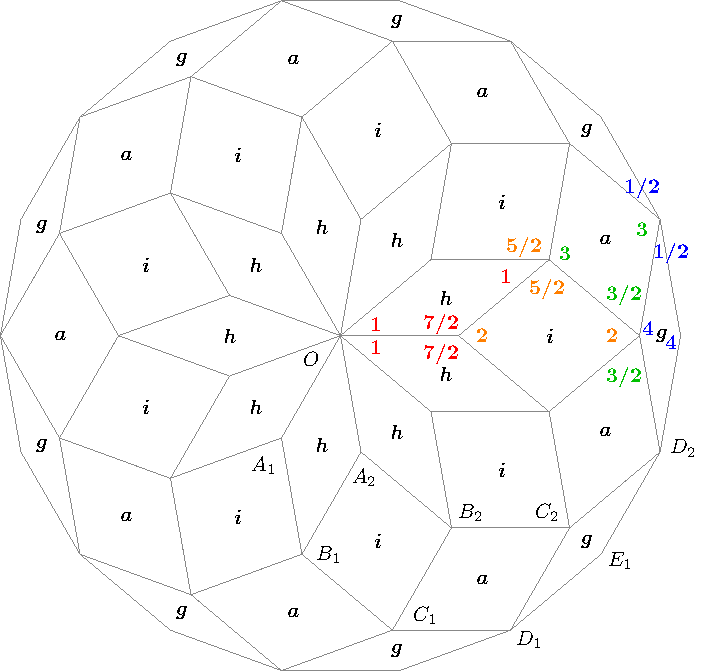
\includegraphics[scale=1]{rhombi-9}
\caption{The symmetry $9$ four rhombi $\{\mathbi{h},\mathbi{i},\mathbi{a},\mathbi{g}\}$ produce the four stars $\{\mathcal{G},\mathcal{H},\mathcal{I},\mathcal{J}\}$ with areas
$9\mathbi{h}$,
 $9(\mathbi{h}+\mathbi{i})$,
 $9(\mathbi{h}+\mathbi{i}+\mathbi{a})$ and 
 $9(\mathbi{h}+\mathbi{i}+\mathbi{a}+\mathbi{g})$ respectivelly.}
\label{fig:rhombi-9}
\end{figure}





\section{Hexagons}

For any odd symmetry $s$, we can obtain equilateral hexagons by connecting six equal edges at integral values of $u$ or by adding and substracting rhombi or by dissecting the areas left after stars intersections. In any case we find the hexagons has at most three different internal angles in this order $(u_1, u_2, u_3, u_1, u_2, u_3)$ where $u_1 + u_2 + u_3 = s$.

\subsection{Hexagons angles}

Figure \ref{tbl:hexagons-angles} show the hexagons defined as $H_s(u_1,u_2)$ for symmetries $s = \{3,5,7,9\}$ where $u_1 \leq u_2 \leq u_3$. We labeled the non self-intersecting hexagons with uppercase letters $\mathbi{A}$, $\mathbi{B}$, $\mathbi{C}$, ... We prevent to name differently any hexagon which is equivalent to a previous one having the same angles as what happens with hexagon $\mathbi{A}$ of symmetries $3$ and $9$.

\begin{table}[H]
\begin{center}
\begin{tabular}{| c | c | c | l | }
\hline
$H_s(u_1,u_2)$ & Label & $(u_1, u_2, u_3)$ & Polygon \\ \hline\
$H_3(1,1)$ & \mathbi{A} & (\textbf{1, 1, 1}) & Regular hexagon \\[0.5ex]
\hline
$H_5(1,1)$ & \mathbi{B} & (\textbf{1, 1, 3}) & Sormeh Dan Girih tile\\[0.5ex]
$H_5(1,2)$ & \mathbi{C} & (\textbf{1, 2, 2}) & Shesh Band Girih tite\\[0.5ex]
\hline
$H_7(1,1)$ & -          & (\textbf{1, 1, 5}) & self-intersecting \\[0.5ex]
$H_7(1,2)$ & \mathbi{D} & (\textbf{1, 2, 4}) & \\[0.5ex]
$H_7(1,3)$ & \mathbi{E} & (\textbf{1, 3, 3}) & \\[0.5ex]
$H_7(2,2)$ & \mathbi{F} & (\textbf{2, 2, 3}) & \\[0.5ex]
\hline
$H_9(1,1)$ & -          & (\textbf{1, 1, 7}) & self-intersecting \\[0.5ex]
$H_9(1,2)$ & \mathbi{G} & (\textbf{1, 2, 6}) & \\[0.5ex]
$H_9(1,3)$ & \mathbi{H} & (\textbf{1, 3, 5}) & \\[0.5ex]
$H_9(1,4)$ & \mathbi{I} & (\textbf{1, 4, 4}) & \\[0.5ex]
$H_9(2,2)$ & \mathbi{J} & (\textbf{2, 2, 5}) & \\[0.5ex]
$H_9(2,3)$ & \mathbi{K} & (\textbf{2, 3, 4}) & \\[0.5ex]
$H_9(3,3)$ & \mathbi{A} & (\textbf{3, 3, 3}) & equivalent to $H_3(1,1)$\\[1.1ex]
\hline
\end{tabular}
\caption{Hexagons $H_s(u_1,u_2)$ for symmetries $s = \{3,5,7,9\}$.} 
\label{tbl:hexagons-angles}
\end{center}
\end{table}


\subsection{Hexagons areas}

\begin{figure}[H]
\centering
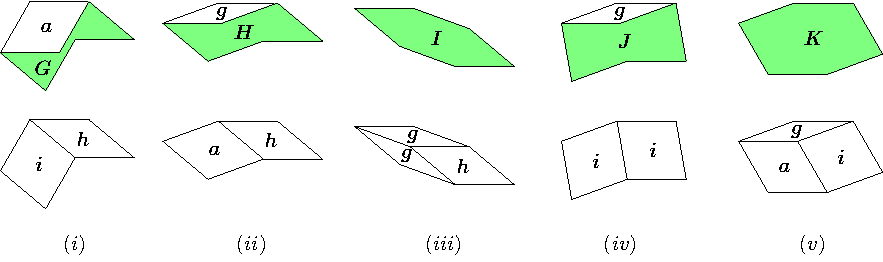
\includegraphics[scale=1]{hexagons-from-rhombi-9}
\caption{Symmetry $9$ hexagons formed adding and substracting rhombi.}
\label{fig:hexagons-from-rhombi-9}
\end{figure}

Figure \ref{fig:hexagons-from-rhombi-9} show how to calculate the area of the symmetry $9$ hexagons in function of the symmetry $9$ rhombi. From $(i)$ to $(vi)$ we equate the area of sum of the polygons in the top with the area of the sum of the polygons of the bottom. We have for the six cases these six equations:
\begin{align}
\mathbi{a} + \mathbi{G} &= \mathbi{i} + \mathbi{h} \\
\mathbi{g} + \mathbi{H} &= \mathbi{a} + \mathbi{h} \\
\mathbi{I} &= 2\mathbi{g} + \mathbi{h} \\
\mathbi{g} + \mathbi{J} &= 2\mathbi{i} \\
\mathbi{K} &= \mathbi{g} + \mathbi{a} + \mathbi{i} \\
\mathbi{A} &= 3\mathbi{a}
\end{align}

\begin{figure}[H]
\centering
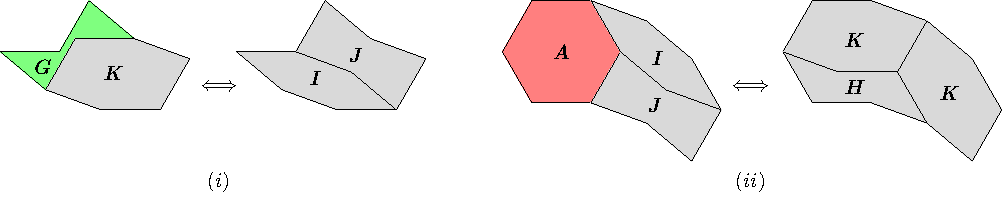
\includegraphics[scale=1]{hexagons-from-hexagons-9}
\caption{Hexagons $\{\mathbi{G},\mathbi{A}\}$ formed adding and substracting hexagons $\{\mathbi{H},\mathbi{I},\mathbi{J},\mathbi{K}\}$.}
\label{fig:hexagons-from-hexagons-9}
\end{figure}

Figure \ref{fig:hexagons-from-hexagons-9} show how to express the area of the six hexagons in function of only four. For $(i)$ and $(ii)$ we equate the area of the sum of hexagons of the left with the area of the hexagons of the right. We have for the two cases these two equations:
\begin{align}
\mathbi{G} + \mathbi{K} &= \mathbi{I} + \mathbi{J} \\
\mathbi{A} + \mathbi{I} + \mathbi{J} &= \mathbi{H} + 2\mathbi{K}
\end{align}

Using the last eight equations we form the table \ref{tbl:hexagons-areas} which show the areas of the six hexagons in function of four rhombi $\mathbi{g,h,a,i}$ and in function of only four hexagons $\mathbi{H,I,J,K}$.

\begin{table}[H]
\begin{center}
\begin{tabular}{| c | l | l |}
\hline
Hexagon & $\mathbi{g,h,a,i}$ area & $\mathbi{H,I,J,K}$ area \\ \hline\
$\mathbi{H}$ & $\mathbi{a} + \mathbi{h} - \mathbi{g}$ & $\mathbi{H}$ \\[0.5ex]
$\mathbi{I}$ & $2\mathbi{g} + \mathbi{h}$ & $\mathbi{I}$ \\[0.5ex]
$\mathbi{J}$ & $2\mathbi{i} - \mathbi{g}$ & $\mathbi{J}$ \\[0.5ex]
$\mathbi{K}$ & $\mathbi{g} + \mathbi{a} + \mathbi{i}$ & $\mathbi{K}$ \\[0.5ex]
\hline
$\mathbi{A}$ & $3\mathbi{a}$ & $2\mathbi{K} + \mathbi{H} - \mathbi{I} - \mathbi{J}$ \\[0.5ex]
$\mathbi{G}$ & $\mathbi{i} + \mathbi{h} - \mathbi{a}$ & $\mathbi{I} + \mathbi{J} - \mathbi{K}$ \\[0.5ex]
\hline
\end{tabular}
\caption{Symmetry $9$ hexagon areas.} 
\label{tbl:hexagons-areas}
\end{center}
\end{table}


\subsection{Hexagons from stars}

Figure \ref{fig:hexagons-9} show the disposition of the symmetry $9$ four stars. We label the $18$ vertices of stars $\{\mathcal{G},\mathcal{H},\mathcal{I},\mathcal{J}\}$ as
 $\{G_0,G_1,...,G_{17}\}$,
 $\{H_0,H_1,...,H_{17}\}$,
 $\{I_0,I_1,...,I_{17}\}$ and
 $\{I_0,G_1,...,I_{17}\}$ respectivelly. 
For simplicity, only some vertices are show. First we make coincident at vertice $O$ all the vertices $G_0,H_0,I_0,J_0$. With the center at $O$ we rotate all stars to make coincidents
$G_{17}$, $H_{17}$, $I_{17}$ and $J_{17}$. The rotations also joined another different vertices.

First we add three new edges (in red) joining the stars $\mathcal{J}$ and $\mathcal{I}$ vertices: $\overline{J_3I_2}$, $\overline{J_5I_4}$ and $\overline{J_7I_6}$ dissecting the red region into four hexagons, two of them essentially different. The three consective angles of the two hexagons are shown: $\textbf{I (1,4,4)}$ and $\textbf{K (3,4,2)}$.

Then we add three new edges (in orange) joining the stars $\mathcal{I}$ and $\mathcal{H}$ vertices: $\overline{I_3H_2}$, $\overline{I_5H_4}$ and $\overline{I_7H_6}$ dissecting the orange region into four hexagons, two of them new. The three consective angles of the the two hexagons are show: $\textbf{H (1,5,3)}$ and $\textbf{A (3,3,3)}$.

Finally we add three more edges (in green) joining the stars $\mathcal{H}$ and $\mathcal{G}$ vertices:
$\overline{H_3G_2}$, $\overline{H_5G_4}$ and $\overline{H_7G_6}$ dissecting the green region into four hexagons, two of them new. The three consective angles of the the two hexagons are show: $\textbf{G (1,6,2)}$ and $\textbf{J (2,5,2)}$.


\begin{figure}[H]
\centering
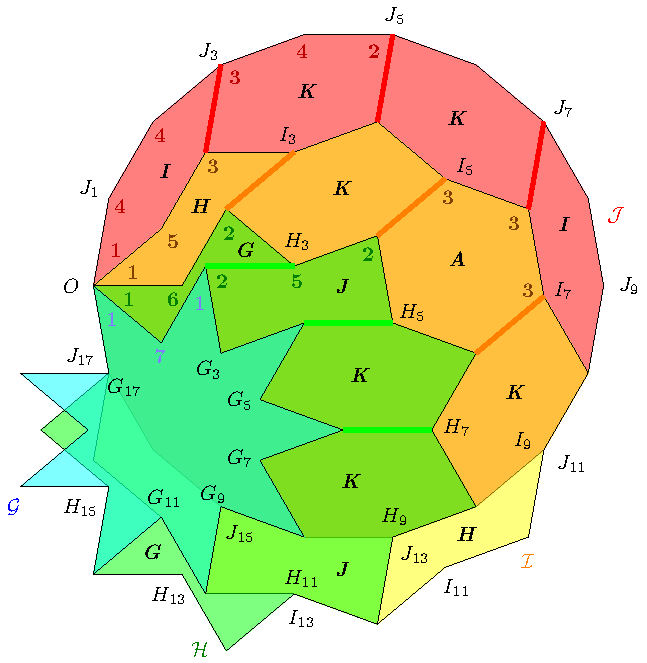
\includegraphics[scale=1]{hexagons-9}
\caption{Symmetry $9$ stars $\{\mathcal{G},\mathcal{H},\mathcal{I},\mathcal{J}\}$
 dissected to get the six hexagons
$\{\mathbi{G},\mathbi{H},\mathbi{I},\mathbi{J},\mathbi{K},\mathbi{A}\}$.
}
\label{fig:hexagons-9}
\end{figure}

\section{Octagons}

\subsection{Octagons by stars}

\begin{figure}[H]
\centering
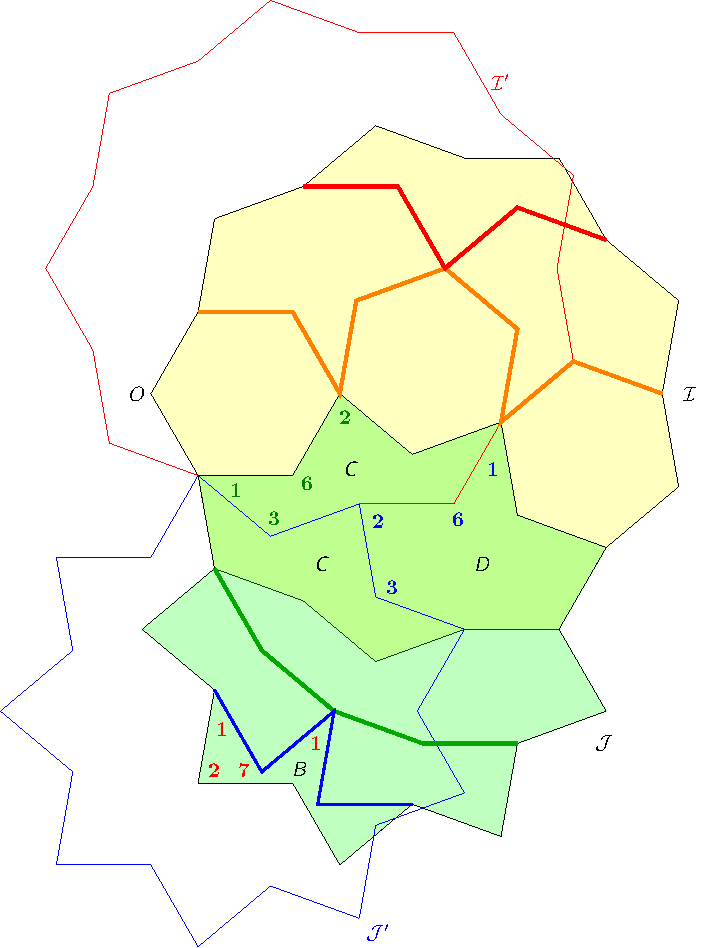
\includegraphics[scale=1]{octagons-9}
\caption{Octagons after intersection of stars $\mathcal{I}$ and $\mathcal{J}$.}
\label{fig:octagons-9}
\end{figure}

%\section{Vectors}
%\begin{figure}[H]
%\centering
%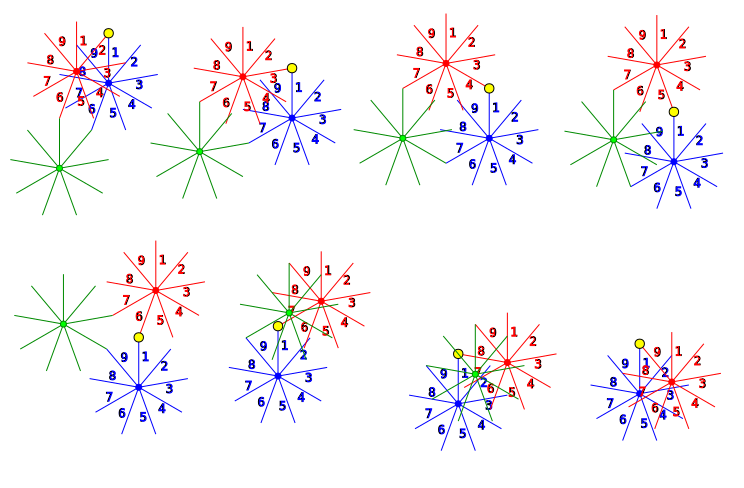
\includegraphics[scale=0.85]{9}
%\caption{Vectors of symmetry $9$.}
%\label{fig:9}
%\end{figure}

\end{document}

